We test the feasibility of the idea with numerical 
simulations. 
To quantify how well the algorithm perform, we employ a quantity r to show the tightness of correlation.
\begin{eqnarray}
	r\equiv \frac{P_{recon,real}}{\sqrt{P_{recon}P_{real}}}\,
\end{eqnarray}

We employ an ensemble of six $N$-body simulations from the
$\mr{CUBEP}^3\mr{M}$ code \cite{2013:code}. 
Each simulation includes $2048^3$ particles in a $(1.2\mr{Gpc}/h)^3$ box. 
%with following cosmological parameters: Hubble parameter $h=0.678$, baryon
%density $\Omega_{b}=0.049$, dark matter density $\Omega_{c}=0.259$,
%amplitude of primordial curvature power spectrum $A_s=2.139\times10^{-9}$ at 
%$k_0=0.05\;\mr{Mpc}^{-1}$ and scalar spectral index $n_s=0.968$.
In the following analysis we use outputs at $z=1$.

For simplicity, we assume the experimental
noise to be zero above a cut off scale and infinity below the cut off scale.
This is a reasonable approximation for a filled aperture experiment, which
has good brightness sensitivity and an exponetially growing noise at small 
scales.
We choose this scale to be $k_c=0.5\ h/\mr{Mpc}$, which corresponds
to $\ell=1150$ at $z=1$. This is realistic for the ongoing 21cm experiments like
CHIME \cite{2014SPIE.9145E..22B}\cite{2014SPIE.9145E..4VN}
and Tianlai \cite{2012IJMPS..12..256C}\cite{2015ApJ...798...40X}.
\tcb{copied}

To mimic the influence of foreground substraction, we use a high pass filter 
$W_{fs}(k_\parallel)=1-e^{-k_\parallel^2R_\parallel^2/2}$. We choose 
$R_\parallel=15\ \mr{Mpc}/h$, which gives
$W_{fs}=0.5$ at
$k_\parallel=0.08\ \mr{Mpc}/h$.
This corresponds to the condition of current 21cm observations  
\cite{2013ApJ...763L..20M}\cite{Switzer13}.

The observed 21cm field after foreground subtraction is given by 
\begin{eqnarray}
\delta_{fs}(\bm{k})=\delta(\bm{k})W_{fs}(k_\parallel)\Theta(k_c-k),
\end{eqnarray}
where $\delta(\bm{k})$ is the density field from simulations, $W_{fs}$ accounts for 
the effect of foreground subtraction and $\Theta(x)$ is the step function 
which equals $1$ for $x\ge0$ and otherwise $0$.
Then we get the reconstructed clean field $\hat \kappa_c$ from $\delta_{fs}$ via
cosmic tidal reconstruction. 
Using $\hat \kappa_c$ we obtain an estimate radial velocity field $\hat v_z$ as in Eq.(\ref{eq:v}).
And then we reconstruct the kSZ signal following Eq.(\ref{eq:ksz}) and compare it with the kSZ signal from simulations.

\begin{figure}[tbp]
	\begin{center}
		\includegraphics[width=0.48\textwidth,height=0.52\textheight]{powermomen_correlation.eps}
	\end{center}
	\vspace{-0.7cm}
	\caption{(Top)$P_{kSZ}$: powerspectrum of orginal kSZ signal $\Theta$, 
		$P_{21cm}$: powerspectrum of reconstructed kSZ signal from foreground substracted 21cm field with $R_\parallel = 15$ Mpc/h, after tidal reconstruction; 
		$P_{cross}$ the cross powerspectrum of this two fields; 		

		(Bottom) The correlation coefficient r between reconstructed kSZ signal and original kSZ signal.
	}
\label{fig:kSZ}
\end{figure}


